\documentclass{styles/llncs} 
%\usepackage{times}
%\usepackage[margin=1in, paperwidth=8.5in, paperheight=11in]{geometry}

% bib stuff
\usepackage{cite}
\usepackage{balance}

%\pagestyle{empty}

% math fonts
\usepackage{amstext}
\usepackage{amsfonts} 
\usepackage[cmex10]{amsmath}
% fix the math symbols that the usenix style (mathptmx) changed
\DeclareMathAlphabet{\mathcal}{OMS}{cmsy}{m}{n}
\interdisplaylinepenalty=2500

% paths and extensions for graphic files
\usepackage{graphicx}
\usepackage[outdir=figures/]{epstopdf}
\graphicspath{{figures/}}
% \DeclareGraphicsExtensions{.pdf}

\usepackage{floatflt}
\usepackage[caption=false,font=footnotesize]{subfig}
%\captionsetup[subfloat]{listofformat=parens}

% tables
\usepackage{tabularx}
\usepackage{multirow}
%\usepackage{multicol} 

\usepackage{url}
\usepackage{xspace}
\usepackage[usenames,dvipsnames]{color}

% label the appendices
%\usepackage{appendix}

% reduce space between bib items
% \usepackage{natbib}
% \setlength{\bibsep}{1pt}

% add line numbers for feedback purposes
% \usepackage{lineno}
% \setpagewiselinenumbers
% \modulolinenumbers[1]
% \linenumbers

% Using watermark (this will mess up top/bottom margins)
\usepackage{styles/pdfdraftcopy}
\draftcolor{gray20}
\draftstring{
\begin{minipage}{17cm}
\begin{center}
\  DRAFT - \today
\end{center}
\end{minipage}
}

\draftfontsize{36pt}

% should be loaded last (but before algorithm*) -colored links and refs
\usepackage[colorlinks=true, citecolor=OliveGreen, linkcolor=BrickRed, urlcolor=MidnightBlue, final, pdftex]{hyperref}

\hypersetup{
    pdfauthor={Bryan Ford, Miles Richardson, Mainak Ghosh},
    pdfsubject={TorCoin},
    pdftitle={},
    pdfkeywords={Incentive, Monetize, Anonymity, Tor}
}

\usepackage{algorithm}
\usepackage{algorithmic}

% space between sections
\renewcommand{\subparagraph}{} % needed to get titlesec to compile
\usepackage[small,compact]{titlesec}
\titlespacing{\section}{0pt}{3mm plus 1mm minus 1mm}{2mm plus 1mm minus 1mm}
% \titlespacing{\subsection}{0pt}{2mm plus 1mm minus 1mm}{1mm plus 1mm minus 1mm}
% \titlespacing{\subsubsection}{0pt}{2mm plus 1mm minus 1mm}{1mm plus 1mm minus 1mm}

% custom commands
\newcommand{\etal}{{\em et al.\ }}
\newcommand{\naive}{na\"{\i}ve }
\newcommand{\point}[1]{\noindent\textbf{#1}.}
\newcommand{\citeme}{\textbf{\color{red}CITE NEEDED! \xspace}}
\newcommand{\checkme}[1][check me]{\textbf{\color{red}NEEDS REVIEW!--{#1} \xspace}}
\newcommand{\todo}[1][check me]{\textbf{\color{red}TODO!--{#1} \xspace}}
\renewcommand{\S}{Section\xspace}
\newcommand{\anote}[1]{{\color{magenta}{#1}}}

% \date{}
\title{TorCoin}

\author{Bryan Ford \and Miles Richardson \and Mainak Ghosh}

\institute{
	Yale University, New Haven, CT\\
	\email{\{bryan.ford, miles.richardson, mainak.ghosh\}@yale.edu}
}

% Alter some LaTeX defaults for better treatment of figures:
% \renewcommand{\textfraction}{0.07}  % allow minimal text w. figs
% \renewcommand{\floatpagefraction}{0.7}  % require fuller float pages
% \renewcommand{\dblfloatpagefraction}{0.7}   % require fuller float pages

\begin{document}

% \pagenumbering{arabic}

% \clubpenalty=9999
% \widowpenalty=9999 

% space between paragraphs
% \setlength{\parskip}{0.5mm plus 0.25mm minus 0.25mm}

\maketitle
%\thispagestyle{empty}

\begin{abstract}
The scalability of the Tor Anonymity Network currently depends on volunteer relay operators for bandwidth. This is unsustainable. We present a method to compensate Tor relay operators and retain anonymity, without charging clients for access. Our solution relies on two novel concepts. First, we introduce \textit{TorCoin}, an ``altcoin'' that uses the BitCoin protocol to reward relays for contributing bandwidth. Relays ``mine'' TorCoins, then sell them for cash on any existing ``altcoin exchange.'' To verify that a given TorCoin represents actual bandwidth transferred, we introduce \textit{TorPath}, a decentralized protocol for assigning Tor circuits to clients, such that each is privately-addressable but publicly verifiable. [ADD TO THIS WHEN THE PAPER IS DONE]
\end{abstract}

\section{Introduction}

Tor is the most popular deployed anonymous communication system, currently
transferring over 8 GiB/s in aggregate~\cite{tornetmet}. The bandwidth that Tor
requires to function is donated by altruistic volunteers at a cost without any
direct return on their investment. As a result, Tor has primarily grown through
the use social and political means. It is a commonly held belief in the Tor
community that utilizing volunteer resources without providing an incentive to
contribute is not a viable long-term strategy for growing the network. How to
recruit new bandwidth providers to the Tor network while maintaining anonymity
is a well studied problem~\cite{raykova-pet2008, wpes09-xpay, incentives-fc10,
ccs10-braids, acsac11-tortoise, jansen2013lira, johnson2013onions}. However,
none of this work has led to any of a number of practical changes in Tor that
would be required to move to an incentive-based resource model for a variety of
reasons.

This paper has two major goals:
\begin{enumerate}
\item to identify the requirements, challenges, and trade-offs in designing an
incentive scheme for the popular operational Tor Network; and 
\item to propose an incentive-based Tor Network architecture with acceptable
trade-offs while presenting an approach to realizing it with mostly existing
technologies and some additional development.
\end{enumerate}
We hope to illuminate the challenges and research problems in a way that will
provoke useful discussion in the community while creating a useful base for
future research in this area.

We begin in \S\ref{reqs} by identifying the requirements and challenges involved
in designing an incentive scheme for Tor while discussing the potential impacts
that various design decisions may have on the existing network and its
operators. We then propose a technical architecture based on existing
technologies in \S\ref{arch}, discuss related work in \S\ref{rel}, and present
several remaining research problems while concluding in \S\ref{conc}.
%\section{Background Information}

\subsection{Why is Internet Anonymity Important?}

The past decade has seen unprecedented empowerment of global citizens. Never before has it been so easy to share, communicate, and collaborate. Less than a century ago, sending a simple photo from China to the United States took weeks or months. Now, with the press of a button on a mobile phone, a single person in China can distribute a video to millions across the globe in a matter of seconds.

This movement is catching authoritarian governments off-guard, because the Internet allows dissent to spread virally throughout populations. The Arab Spring exemplified government resistance to mass dissent. In an attempt to stop it, the governments employed heavy-handed measures like blocking social media. Fortunately, anonymity technologies rendered them fruitless. As such, improving anonymity technologies remains a subject of utmost importance.

\subsection{Tor provides anonymity and censorship resistance.}

Anonymity ensures that power stays in the hands of citizens, not the government. Specifically, the Tor project's routing protocol enables anonymity through a special onion routing protocol. It routes requests through thousands of volunteer nodes such that no node or outside observer can de-anonymize the request. This protocol ensures anonymity between all nodes on the network, and incidentally allows users to circumvent censorship because no entity can know their destinations. Tor is a great tool for ensuring anonymity and resisting censorship.

\subsection{Tor is great, but slow.}

Tor is slow, as a result of oversubscription to the Tor network. Only one Tor network exists, and it depends on volunteers to supply server hardware and bandwidth. Unfortunately, Tor is too popular! More people want to use it than the servers can support. So, essentially, the Tor network suffers from a shortage of relay servers. The obvious explanation for the shortage is a lack of incentive to supply the servers. Volunteers actually pay a cost to assume a risk. They supply expensive bandwidth and servers, in exchange for nothing except the fear of an FBI battering ram smashing through their doors. This lack of economic incentive represents a fundamental flaw in the Tor network. Tor will never become mainstream without enough servers to support more users, and it seems there are not enough willing volunteers to provide sufficient servers. So we need to introduce an economic incentive to hosting Tor relay servers.

%\section{Introduction}

\subsection{Launching a Secondary Tor Network}

We will build a system that enables deployment of a secondary, monetized Tor network. Independent communities can launch a private or public network that routes traffic over Tor. In exchange for supplying bandwidth, relay servers receive a special cryptocurrency called a TorCoin.

\subsection{TorCoin Mining}

Relay servers mine TorCoins proportionally to the bandwidth they supply. This mining is analagous to Bitcoin mining, except its proof-of-work scheme is bandwidth-intensive instead of CPU-intensive. As such, a TorCoin represents bandwidth that was pushed over some relay server, somewhere in the Tor network, at some point in time. Therefore, TorCoins have inherent value, because relay operators can trade them in for cash. 

\subsection{Exchanging TorCoins for Cash}

\subsubsection{TorCoins are Valuable to Both Clients and Outsiders}

A TorCoin has value to both clients and outsiders. For clients, a TorCoin has value because it represents bandwidth, which they demand and relays supply. For outsiders, TorCoin has value as an alternative cryptocurrency, also known as an “altcoin.” Increasingly, people are trading altcoins for arbitrage opportunities, money transferring vehicles, and speculative investment. So in this sense, TorCoin is similar to Namecoin, Zerocoin, and any other number of altcoins. 

Because a TorCoin has value to both clients and outsiders, relays have two counterparties for exchanging Torcoins.

\subsubsection{1. Charge clients for access to network}

One can imagine a scheme in which clients must pay a price, in traditional currency (or even Bitcoin), to access the network. Some mechanism then transfers the traditional currency to the relays, in exchange for Torcoins, which the client can use to connect to the network. That is, any client connecting to the network must pay some number of TorCoins. 

In this scenario, we have an open question: What happens to the Torcoins that the clients pay to the network? Relays already received cash for mining them and then selling them to clients via the exchange, so should they get the TorCoins back? This seems to be an ecomomic question, and a difficult one at that. So perhaps this next solution is a better one, as it's much more analagous to Bitcoin.

\subsubsection{2. Keep Tor free, sell TorCoins to AltCoin traders}

Because TorCoins have value outside of the relay-client relationship, they can also be exchanged outside of it. For example, relays who mine Torcoins could sell them on an Altcoin exchange, where traders set the price by trading amongst each other. Thus, relays can exchange Torcoins for cash without the client needing to pay for access to the network. Economically, this works because the relays create value by supplying anonymous bandwidth to clients, and then traders pay for that value as the supply of Torcoins grows.

(This leads us to an important question: Is the supply of Torcoins finite? Much of the appeal of Bitcoins and Altcoins is their finite money supplies. But if Torcoins have a finite money supply, then eventually no more can be mined. Then there is no more incentive for relays to supply bandwidth. So, we have a catch-22. We need to always incentivize relays to provide bandwidth, but Altcoin traders prefer currencies with finite money supplies. One possible solution to this is to reset the money supply every time it reaches its limit -- or even to launch a new Altcoin each time.)
%\section{Requirements} \label{reqs}

A Tor incentive system that rewards volunteers for providing useful network
services presents numerous requirements and challenges, both technical and
social. In this section we briefly identify the major technical problems that we
believe such a system should solve, while noting that all of the solutions
should happen ``offline" so as to minimize the interference with Tor's
low-latency communication design. Please see \S\ref{disc} for a discussion of
the social challenges involved in deploying a Tor incentive system.

\paragraph{Proofs of Useful Service} A system that rewards users for serving the
network should be able to prove that those services were in fact rendered.
Ideally, the proofs of service would be publicly verifiable so that any member
of the distributed network could validate the utility provided by any other
member.

\paragraph{Rewards for Providing Service} Members that contribute to the system
should be rewarded for their contributions in proportion to the amount that was
contributed. Ideally, the reward should have internal value in that a member can
use it to achieve a desirable system service or attribute.

\paragraph{Accountability} The system should provide a way to account for the
rewards obtained by each member, and provide facilities to exchange rewards for
desirable services. Double spending of rewards should be prevented or detected
and handled. Ideally, the process of accounting for rewards should be publicly
verifiable in order to eliminate reliance on centralized entities.

\paragraph{Preserve Anonymity} The system should not introduce new attacks
on the anonymity Tor offers to its users. As such, the solution to providing
accountability and exchange of rewards should not link users to their past
network usage activities.

\paragraph{Deployability} The system should integrate well with the existing Tor
network in order to maximize the utility provided to existing users and leverage
the existing infrastructure and community. Ideally, the system components will
be modular to allow them to be incrementally deployed with the existing Tor
network.

%% old stuff left in in case it's useful at some point
%\section{Requirements, Challenges, Trade-offs, and Discussion} \label{reqs}
%
%The Tor incentive approach outlined in our introduction presents numerous requirements and challenges, both technical and social. Here we describe the issues. We assert that building on the Bitcoin protocol allows us to 
%
%\subsection{Basic, High-Level Requirements}
%
%\subsubsection{Secure Bandwidth Measurement}
%
%\begin{itemize}
%\item How do we know a TorCoin really represents proof of bandwidth?
%\item Discuss Eigenspeed.
%\item Needs to work for all circuit positions.
%\item A solution will need to account for bandwidth in both directions through a circuit, and work for all circuit positions
%\end{itemize}
%
%\subsubsection{Account Management}
%
%\begin{itemize}
%\item How do relays present the amount of bandwidth they have contributed? 
%\subitem Answer: Torcoin relies on the Bitcoin protocol for its distributed ledger.
%\item Need some way to manage account for relays, to represent amount of bandwidth they have contributed
%\item All interaction with account management system should happen offline (not part of circuit construction phase, to avoid blocking behavior in Tor)
%\end{itemize}
%
%\subsubsection{Preserve Anonymity}
%
%\begin{itemize}
%\item TorCoin implementation can not reduce anonymity.
%\end{itemize}
%
%\subsubsection{Exchange Mechanism}
%
%\begin{itemize}
%\item System needs to either exist, or be possible, for exchanging Torcoins for cash
%\item Without this system, Torcoins do not represent true incentive to provide bandwidth
%\item Because bandwidth costs cash (pay ISP's)
%\item Do not necessarily need to implement or introduce system ourselves, but should be at least pluggable
%\end{itemize}
%
%
%\subsection{More content, to be categorized later into sections}
%
%
%\subsubsection{Network Structure}
%
%Central:
%\begin{itemize}
%\item run by a single entity
%\item not resilient to takedowns or malicious behavior
%\item potentially a severe performance bottleneck
%\end{itemize}
%
%Federated:
%\begin{itemize}
%\item runs on existing directory servers using something like opentransactions.org to provide ecash
%\item transactions are instantaneous
%\item relies on small trusted directory server set
%\item communication/performance overhead among bank members means it is not scalable, and it gets more complicated if you need several federated sets to handle different parts of the network
%\end{itemize}
%
%Completely decentralized:
%\begin{itemize}
%\item use an AltCoin or something else as a distributed storage medium for the ledger
%\item more scalable
%\item decentralized trust may not be relevant in Tor's existing trust model, but will be when Tor moves away from federated directory server model
%\item transaction linkability issues leads to protocol complexities and questions about anonymity. does zerocoin work here?
%\end{itemize}
%
%\subsubsection{Trust Assumptions}
%
%trusted, honest but curious, untrusted.
%
%\subsection{Incentives to Participate}
%
%We can use performance enhancements as an incentive, which may lead to monetary value if a generic 'coin' or other token is used that can be traded among clients. There may be designs where exchanging coins is not possible, and so the coin would have no value to others.
%
%Differentated Services~\cite{Blake1998}.
%
%\subsubsection{Guaranteed Quality of Service}
%
%\subsubsection{Differentiated Service}
%
%Differentated Services~\cite{Blake1998}.
%
%\subsection{Integration with the Tor Network}
%
%If it is run outside of Tor it may be better for experimental purposes, but longer term it would be nice not to partition the network.
%
%How do these options this affect the anonymity sets? Will it always be possible to split the sets anyway due to the fundamental nature of diffserv scheduling?
%
%\subsubsection{Deploy in Existing Tor Network}
%
%Write Tor proposals, get all the new features blessed by the Tor developers, integrate into existing network.
%
%\subsubsection{New and Separate Anonymity Network}
%
%Fork Tor and add the new features. Create a separate network that does not interact with the existing network.
%
%\subsubsection{New Anonymity Network used with Tor}
%
%Run a separate network that is 'attached' to the existing network. In other words, the new network interoperates with Tor by having two consensus files, etc. Then, when people wanting to use the coin mechanism use the new consensus to choose relays from the new network, and non-payers use the Tor consensus to choose circuits in the existing Tor network.
%
%\subsection{Anonymity}
%
%\subsubsection{Transaction Unlinkablity}
%
%Whatever mechanism used to pay relays (ecash, coin, or bank) should provide completely unlinkable transactions in order to maintain Tor's anonymity.
%
%\subsubsection{Partitioning Anonymity Sets}
%
%The anonymity sets of payers vs non-payers should be considered. Is anonymity fundamental to diffserv or a similar approach that is needed to actually create the incentive? In other words, if we use performance differentiation as an incentive, then at some level that can also be used as a distinguisher of who is paying and not paying for service.
%
%\subsection{Diversity}
%
%\subsubsection{Location Diversity}
%
%The market might prefer a single cheap ISP, which would not add additional location diversity to the network. We could create a "diversity weight" and pay more for relays that increase the diversity weight
%
%\subsubsection{Circuit Position Diversity}
%
%Should we pay more for entry or exit position, or for exit policies that are more open by some definition? Or will the market smooth this out automatically?
%
%\subsubsection{Diversity in Capabilities}
%
%We could offer more reward for faster relays (i.e. a super-linear reward scale), or for relays that are running a certain version or support a certain feature (experimental or otherwise). This could improve the community's ability to contribute to decisions about what to support instead of completely relying on the Tor developers (could be a good thing or a bad thing).
%
%\subsection{Community Interaction}
%
%If a new incentive scheme is incorporated into Tor, will existing volunteers stop caring become less altruistic and leave because they will view Tor as a commercial network? Will people lose interest in helping the broader Internet freedom cause?
%
%Does a token that only provides a performance enhancement but has no intrisic value (cannot be traded with others) solve this problem? Or does the fact that you can trade the coins provide most of the incentives?
%
%Would a smaller scale experiment outside of the existing Tor network to test the feasibility of an incentive approach be helpful, or would the conclusions simply be synthetic because users/relays in the experimental network would not have the same ideals and values as in existing network?

\section{Proposed Architecture} \label{arch}

We now discuss the main components necessary to realize a practical Tor
incentive system while identifying some open research and development problems.

\subsection{Overview}
We propose a system that measures bandwidth contributed to the Tor network to produce incentivise the addition of nodes to the Tor network.

The system measures the bandwidth contributed by each relay in the Tor network and rewards them with a 'TorCoin'. A Torcoin is an AltCoin that uses a bandwidth-intensive protocol as its proof-of-work. Thus, to produce a TorCoin, a relay must have transmitted a certain amount of Tor traffic.

To reduce the system's vulnerability to attackers and possible reduction of anonymity, we also utilize a system of 'Ephemeral Paths' to randomly assign relays to clients.

These TorCoins can then be traded at an exchange for other AltCoins or other goods. This forms the basis of our incentivization scheme. This is different from systems that propose differentiated service\cite{dovrolis1999case, dovrolis2002proportional}, since we do not propose to make the clients pay for access to the network. The coins are a byproduct of the usage of the system.

\subsection{Ephemeral Paths}
The TorCoin system adheres to the following constraints:
\begin{itemize}
  \item No client in the group can generate its own route.
  \item Every resulting route has a unique public key (Route signature).
  \item No client in the group can know the route assigned to another client in the group.
  \item Any interested party can verify that a given public key represents a route assigned to a client in the current group.
\end{itemize}

\subsubsection{Setup}
The Tor directory servers will create the groups using the temporal locality of the clients connecting to them, but also ensure that there is geographical and other diversity in a group. This is to ensure that adversaries cannot deterministically place themselves in a single group by connecting at the same time.

A group consists of the first n = 1000 or so clients that have connected to the Assigning servers. In practice, we expect the number n to be modulated so that groups are being created every 10 seconds or so. Also, we will ensure diversity in the group by ensuring that a group consists of a majority of the Assigning servers. Thus, if there are 10 Assigning Servers in the entire network, a group must consist of atleast 6 of them.


\subsubsection{Route Assignment using Neff shuffles}
Once all the clients have filled up the group, the Assigning Servers in the group initiate the process of route assignment.
\begin{enumerate}
  \item Three groups of two Assigning Servers are chosen from those in the group.
  \item Each group of Assigning servers uses a unique Neff shuffle to create shuffled lists of entry, middle and exit relays. The ith client in the group is thus matched up with the ith entry, middle and exit relay to form a 'route'.
  \item The servers then create a route-signature for each route based on some property of each participant (client and three relays).
  \item Each route-signature is then input into a cryptographic accumulator so that anyone can verify if a route belonged to a group. This accumulator is published in a publicly available log along with the timestamp of the group creation.
\end{enumerate}

Each server then sends each client in the group one piece of data. Eg: The servers that assigned the entry relays send each client its ownentry relay. Similarly, the middle and exit relays and the route signatures are also communicated in the same way. 
For each relay, the servers send an Access Control List. This is a list of all the relays and clients that the relay should accept connections from, as well as the route signatures for each.

In this way, no single server is aware of any client's entire path through the network, preserving their anonymity. Since each relay is confirmed by atleast two servers, it is also robust to rogue servers. 

\subsubsection{Proof of Bandwidth - Onion Hashing}
Once the routes are setup, we can prove bandwidth transfer through the following protocol:
Every m Tor packets, the client sends an extra packet (“the Torcoin packet”) containing an hash attempt likely to generate a TorCoin. Relay A gets it, generates a temporary private key Ka (generated using the route shared key) and hashes the received packet and this key. It then forwards it to B, which does the same thing, with its own private temporary key Kb. Similarly on to C. C can now add its own Kc, and if it generates a hash with a given number of zeros, it can claim to have found a TorCoin.
\begin{verbatim}
Client sends to A: T0 (its hash attempt)
A sends to B     : Hash(T0 + K1) = Ta # K1 is A's temporary private key.
B sends to C     : Hash(Ta + K2) = Tb # K2 is B’s temporary private key.
C computes       : Hash(Tb + K3) = Tc # K3 is C’s temporary private key.
C sends to B     : (Tc, K3) to verify.
B sends to A     : (Tc, K3, Tb, K2) to verify.
A sends to client: (Tc, K3, Tb, K2, Ta, K1) to verify.
Once the client has verified the hash, we can confirm that the data has made a 
round trip through the route. This completes the proof of bandwidth.
\end{verbatim}

\subsubsection{TorCoin}
We can then implement an AltCoin based on the proof-of-work concept in the following manner:
\begin{verbatim}
If (Tc = '000...')
  If the client succesfully verifies the hash
    It adds the coin to the blockchain with the following information:
    0. Timestamp of group.
    1. Client’s public key.
    2. Route Shared key (Lets any other group member verify that the route is 
       genuine. See accumulator.)
    4. TorCoin Hash.
    It then gives 1/3rd of the coin to each of the relays in the route. (If the 
    client is rogue, can we identify and kick the client off?)
\end{verbatim}
This information in the blockchain will enable any interested party to verify if the route came from a legitimate group formed by the directory servers. This can be done by taking the route signature and comparing it with the publicly available accumulators. 

The properties of the Altcoin will then take over, with clients building on the blockchain with more and more TorCoins that they mine through this process.

\subsection{Robustness to attack}
The entire reason for constructing the elaborate ephemeral routes algorithm is to make the Torcoin system robust to attackers.

Due to the random group selection system, it is hard for attackers to deterministically place themselves in a group. To make the system even more secure, the servers can randomize group assignment instead of just taking temporal locality to be the criterion.

In addition, because the attacker needs to control all four components of a route to mint a TorCoin fraudulently, even if the adversaries control up to half the network, there is a probability of only 1/16 that an adversary client gets a path of three colluding relays. In practice, gaining control of half of the entire Tor client and relay network is practically impossible. 

A separate rate-limiting mechanism can be deployed to detect dishonest relays and remove them from the the path selection procedure. An independent verification authority, such as one based on Eigenspeed, could be used to detect these discrepancies.
\section{Preliminary Results}

The TorCoin protocol adds a small amount of overhead to Tor traffic. 
To evaluate this overhead,
we set up a series of servers using the Python Twisted
framework\cite{twisted} to simulate the passing of TorCoin generation and
verification messages through a set of relays.

Assuming that the keys, hashes and signatures are all 32 bytes in length,
the total overhead from one round of successful TorCoin mining (i.e., one entire
round trip from client through all the relays and back again) results in a total
TorCoin packet overhead of 814 bytes. This can be broken down into:

\begin{itemize}
	\item The first packet from client to entry relay: 34 bytes.
	\item Packet forwarded from entry to middle relay: 66 bytes.
	\item Packet forwarded from middle to exit relay: 98 bytes.
	\item Packet from from exit to middle relay: 164 bytes.
	\item Packet from from middle to entry relay: 194 bytes.
	\item Packet from from entry relay to client: 258 bytes.
	\item Total: 814 bytes
\end{itemize}

\section{Preliminary Results}

The TorCoin protocol adds a small amount of overhead to Tor traffic. 
To evaluate this overhead,
we set up a series of servers using the Python Twisted
framework\cite{twisted} to simulate the passing of TorCoin generation and
verification messages through a set of relays.

Assuming that the keys, hashes and signatures are all 32 bytes in length,
the total overhead from one round of successful TorCoin mining (i.e., one entire
round trip from client through all the relays and back again) results in a total
TorCoin packet overhead of 814 bytes. This can be broken down into:

\begin{itemize}
	\item The first packet from client to entry relay: 34 bytes.
	\item Packet forwarded from entry to middle relay: 66 bytes.
	\item Packet forwarded from middle to exit relay: 98 bytes.
	\item Packet from from exit to middle relay: 164 bytes.
	\item Packet from from middle to entry relay: 194 bytes.
	\item Packet from from entry relay to client: 258 bytes.
	\item Total: 814 bytes
\end{itemize}

\section{Preliminary Results}

The TorCoin protocol adds a small amount of overhead to Tor traffic. 
To evaluate this overhead,
we set up a series of servers using the Python Twisted
framework\cite{twisted} to simulate the passing of TorCoin generation and
verification messages through a set of relays.

Assuming that the keys, hashes and signatures are all 32 bytes in length,
the total overhead from one round of successful TorCoin mining (i.e., one entire
round trip from client through all the relays and back again) results in a total
TorCoin packet overhead of 814 bytes. This can be broken down into:

\begin{itemize}
	\item The first packet from client to entry relay: 34 bytes.
	\item Packet forwarded from entry to middle relay: 66 bytes.
	\item Packet forwarded from middle to exit relay: 98 bytes.
	\item Packet from from exit to middle relay: 164 bytes.
	\item Packet from from middle to entry relay: 194 bytes.
	\item Packet from from entry relay to client: 258 bytes.
	\item Total: 814 bytes
\end{itemize}

\input{figures/tex/results.tex}

Each round of TorCoin generation and verification happens only after $m$ Tor
packets have been sent. Each standard Tor cell is 514 bytes long, so each
round trip on the network requires transmission of 514 * 6 = 3084 bytes. Thus,
if $m \geq 10$, the TorCoin protocol overhead is around 2\%. The value of $m$
can be calibrated in further experimentation and as needed in order to achieve
the sweet-spot of transmission efficiency and incentive maximization for relay
providers.

The system might decrease the value of $m$ when load is high,
incentivizing relay operators
to provision more relay bandwidth at such times.

While the Neff shuffle is complex and requires several
communications between the servers,
we expect the assignment servers will be few (less than 10)
and well-provisioned,
and do not expect the shuffles to be a major bottleneck.
Since this is a one-time cost of connecting to the network,
we hope users will accept this setup time
if it gives them access to higher-capacity relays.
For impatient users,
the TorCoin client could use conventional Tor circuits immediately on startup,
then transition to TorCoin circuits as they become available.



Each round of TorCoin generation and verification happens only after $m$ Tor
packets have been sent. Each standard Tor cell is 514 bytes long, so each
round trip on the network requires transmission of 514 * 6 = 3084 bytes. Thus,
if $m \geq 10$, the TorCoin protocol overhead is around 2\%. The value of $m$
can be calibrated in further experimentation and as needed in order to achieve
the sweet-spot of transmission efficiency and incentive maximization for relay
providers.

The system might decrease the value of $m$ when load is high,
incentivizing relay operators
to provision more relay bandwidth at such times.

While the Neff shuffle is complex and requires several
communications between the servers,
we expect the assignment servers will be few (less than 10)
and well-provisioned,
and do not expect the shuffles to be a major bottleneck.
Since this is a one-time cost of connecting to the network,
we hope users will accept this setup time
if it gives them access to higher-capacity relays.
For impatient users,
the TorCoin client could use conventional Tor circuits immediately on startup,
then transition to TorCoin circuits as they become available.



Each round of TorCoin generation and verification happens only after $m$ Tor
packets have been sent. Each standard Tor cell is 514 bytes long, so each
round trip on the network requires transmission of 514 * 6 = 3084 bytes. Thus,
if $m \geq 10$, the TorCoin protocol overhead is around 2\%. The value of $m$
can be calibrated in further experimentation and as needed in order to achieve
the sweet-spot of transmission efficiency and incentive maximization for relay
providers.

The system might decrease the value of $m$ when load is high,
incentivizing relay operators
to provision more relay bandwidth at such times.

While the Neff shuffle is complex and requires several
communications between the servers,
we expect the assignment servers will be few (less than 10)
and well-provisioned,
and do not expect the shuffles to be a major bottleneck.
Since this is a one-time cost of connecting to the network,
we hope users will accept this setup time
if it gives them access to higher-capacity relays.
For impatient users,
the TorCoin client could use conventional Tor circuits immediately on startup,
then transition to TorCoin circuits as they become available.


%\section{Discussion} \label{disc}

\todo[this section is currently merely an outline of topics for discussion]

\subsection{Path to Deployment}

If it is run outside of Tor it may be better for experimental purposes, but longer term it would be nice not to partition the network.

How do these options this affect the anonymity sets? Will it always be possible to split the sets anyway due to the fundamental nature of diffserv scheduling?

\subsubsection{Deploy in Existing Tor Network}

Write Tor proposals, get all the new features blessed by the Tor developers, integrate into existing network.

\subsubsection{New and Separate Anonymity Network}

Fork Tor and add the new features. Create a separate network that does not interact with the existing network.

\subsubsection{New Anonymity Network used with Tor}

Run a separate network that is 'attached' to the existing network. In other words, the new network interoperates with Tor by having two consensus files, etc. Then, when people wanting to use the coin mechanism use the new consensus to choose relays from the new network, and non-payers use the Tor consensus to choose circuits in the existing Tor network.

As it is important to minimize the loss in anonymity to the existing Tor users,
we propose the deployment of a secondary experimental Tor network that will
separate the incentive design and its risks from the existing network. Those
participating in the incentive scheme will choose relays from a new consensus
produced by a new set of directory servers, and those that do not with to
participate will use the existing network as usual. This deployment strategy
offers the flexibility of merging the incentive design back into Tor should it
prove beneficial, while minimizing risk should it not.

\subsection{Trust in Network Elements}

The benefits of a system that is capable of moving to a decentralized trust model.

\subsubsection{Federated}

\begin{itemize}
\item runs on existing directory servers using something like opentransactions.org to provide ecash
\item transactions are instantaneous
\item relies on small trusted directory server set
\item communication/performance overhead among bank members means it is not scalable, and it gets more complicated if you need several federated sets to handle different parts of the network
\end{itemize}

\subsubsection{Completely decentralized}

\begin{itemize}
\item use an AltCoin or something else as a distributed storage medium for the ledger
\item more scalable
\item decentralized trust may not be relevant in Tor's existing trust model, but will be when Tor moves away from federated directory server model
\item transaction linkability issues leads to protocol complexities and questions about anonymity. does zerocoin work here?
\end{itemize}

\subsection{Diversity}

\subsubsection{Location Diversity}

The market might prefer a single cheap ISP, which would not add additional location diversity to the network. Could we create a "diversity weight" and pay more for relays that increase the diversity weight?

\subsubsection{Circuit Position Diversity}

Should we pay more for entry or exit position, or for exit policies that are more open by some definition? Or will the market smooth this out automatically?

\subsubsection{Diversity in Capabilities}

Could we offer more reward for faster relays (i.e. a super-linear reward scale)?  Or for relays that are running a certain version or support a certain feature (experimental or otherwise)? This could improve the community's ability to contribute to decisions about what to support instead of completely relying on the Tor developers (could be a good thing or a bad thing).

\subsection{Community}

If a new incentive scheme is incorporated into Tor, will existing volunteers stop caring become less altruistic and leave because they will view Tor as a commercial network? Will people lose interest in helping the broader Internet freedom cause?

Does a token that only provides a performance enhancement but has no intrisic value (cannot be traded with others) solve this problem? Or does the fact that you can trade the coins provide most of the incentives?

Would a smaller scale experiment outside of the existing Tor network to test the feasibility of an incentive approach be helpful, or would the conclusions simply be synthetic because users/relays in the experimental network would not have the same ideals and values as in existing network?
\section{Related Work} \label{rel}

PAR~\cite{raykova-pet2008}, XPay~\cite{wpes09-xpay}, Gold Star~, BRAIDS~\cite{ccs10-braids}, Tortoise~, onions for sale~\cite{johnson2013onions}.

On the economics of anonymity~\cite{Acquisti03onthe}, one-to-n scrip systems~\cite{humbert2011-scrip}.

LIRA~\cite{jansen2013lira}is a lightweight system providing “performance incentives for users to contribute bandwidth to the Tor network.” It uses coins, similar to “in game currency,” to distribute payment. LIRA uses coins which have a tunable probability of being right, and clients can guess lottery tickets with probability, p of being right. 

Eigenspeed~\cite{snader2009eigenspeed} is a peer-to-peer consensus building algorithm for monitoring bandwidth over a network, specifically implemented for Tor. Unfortunately it requires a central authority for computing Principal Component Analysis operations. While we believe these operations could be decentralized, we are not interested in extending Eigenspeed. Instead, we exploit properties of the Bitcoin protocol to allow for bandwidth monitoring that is sufficient to generate payment tickets. However, as mentioned before, Eigenspeed could act as a secondary system to monitor relays and clients that seem to be producing more TorCoins than would be warranted by their speed.  
\section{Conclusions} \label{conc}

We have introduced TorPath, a novel scheme to assign paths to Tor
clients securely and anonymously.
TorPath motivated by the need to verifiably mine TorCoins, a
a BitCoin variant based on measured bandwidth over the Tor network.
The TorCoin protocol is robust to malicious relays and clients
colluding to mint TorCoins without transferring bandwidth.

\com{	This is a very minor optimization,
	not worth mentioning if it's the only "Future Work" listed. -baf
Further work could investigate the use of cryptographic accumulators for circuit
signatures, which could reduce the packet overhead during bandwidth-measurement
and make the protocol more efficient.
}

\subsection*{Acknowledgments}

This material is based upon work supported by the Defense Advanced Research
Agency (DARPA) and SPAWAR Systems Center Pacific, Contract No. N66001-11-C-4018.
This work was supported by the Office of Naval Research.



{ \footnotesize %\scriptsize %\footnotesize %\small
\bibliographystyle{styles/splncs}
\balance\bibliography{references}
}

%\clearpage
% \appendix
%\appendixpage
\section*{Appendices}

\section{Performance Rewards with Differentiated Services}

We now describe how the differentiated services
architecture~\cite{blake1998architecture} can be used to improve the control
over traffic priority in Tor, as previously outlined by
Jansen~\cite{jansenphdthesis}. More specifically, the proportional
differentiation model~\cite{dovrolis1999case} allows for predictable (i.e.,
consistent as load increases) and controllable (i.e., adjustable differentiation) performance between N traffic
classes. The model allows for the configuration of a differentiation parameter
$p_i$ for each class $i$, and enforces the proportional priority of a traffic
quality metric $q$ between all pairs of classes $i$ and $j$ for measurement
timescale $\sigma$ as:
\begin{equation}
\forall i \in [N], \forall j \in [N]: \frac{q_i \left( t, t + \sigma \right)}{q_j \left( t, t + \sigma \right)} = \frac{p_i}{p_j}
\end{equation}
where $p_1 < ... < p_N$ and $p_i/p_j$ defines the quality proportion between
classes $i$ and $j$. The model is well defined when there is enough
traffic in each class to allow a work-conserving scheduler to meet the desired
proportions.

Dovrolis \etal design a scheduler under the proportional differentiation model
using a queuing delay metric~\cite{dovrolis2002proportional}, which in our case
corresponds to Tor cell waiting times. For class $i$, the quality metric $q_i$
combines the queuing delay $D_i(t)$ of the longest waiting cell with the
long-term average delay $\delta_i(t)$  of all previously scheduled cells at time $t$:
\begin{equation}
q_i(t) = D_i(t) \cdot f + \delta_i(t) \cdot (1-f)
\end{equation}
where $f$ is an adjustable fraction that tunes the schedulers ability to react
to short term spikes in delay. When a scheduling decision is to be made at time $t$,
the longest waiting cell from the class with the maximum priority
$P(t) = q(t)/p(t)$ is chosen and scheduled.


Todo - DRAFT NOTES:

This section will detail the economic model and present any lingering questions. There will be another diagram featuring multiple clients, a PSP, and multiple hosts. The diagram below will go into the software architecture section, under a section called ``system design'', followed by a sentence describing each component. Then we will go into detail on the ephemeral paths and TorCoin design, which are part of the TorCoin Minter. The TorCoin trader, wallet, and exchange are all necessary, but not novel in terms of design, so we will spend little time on those.

TODO: Add component to Client, ``TorCoin Minter'' (?)

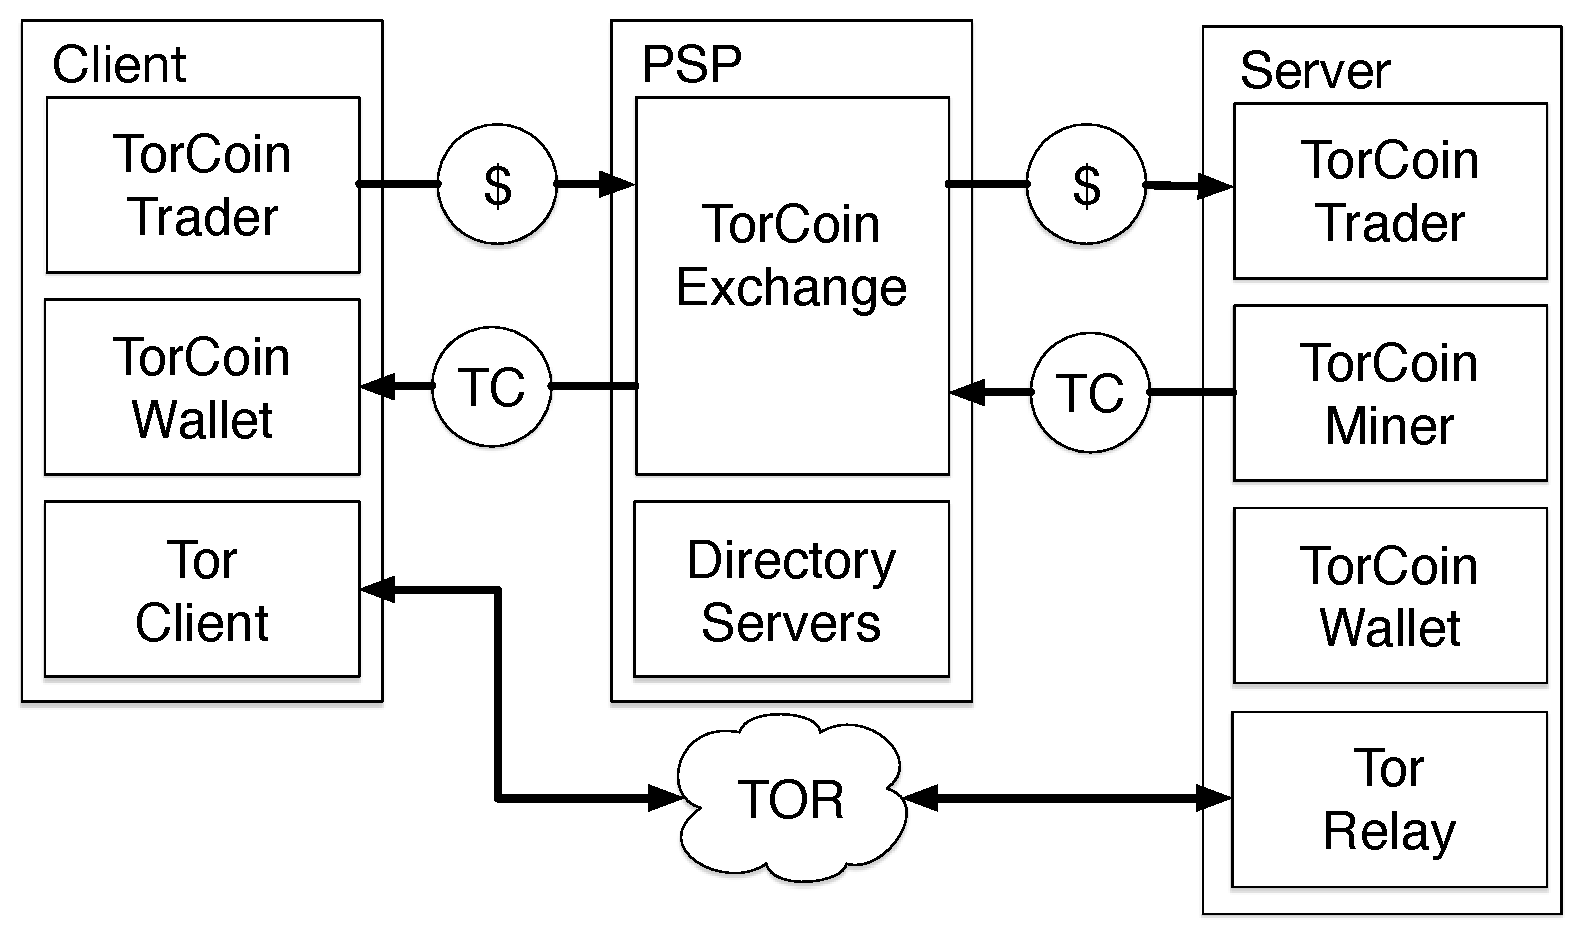
\includegraphics[scale=0.5]{figures/overview.pdf}

\end{document}
